\documentclass[12pt]{article}

\usepackage{algorithm} %pseudo-code
\usepackage{algpseudocode}
\usepackage[top=1in, bottom=1in, left=1in, right=1in]{geometry}
\usepackage{amsmath,amsthm,amssymb}
\usepackage{graphicx}
\usepackage{float}
\usepackage{amsmath, amssymb, amscd}
\usepackage{alltt}
\usepackage{textcomp}
\usepackage{gensymb}
\usepackage{multicol}
\usepackage{tabularx}

\newcommand{\N}{\mathcal{N}}
\newcommand{\Z}{\mathbb{Z}}
\newcommand{\R}{\mathbb{R}}
\newcommand{\bigo}{\mathcal{O}}
\newcommand{\G}{\mathcal{G}}
\newcommand{\V}{\mathcal{V}}
\newcommand{\E}{\mathcal{E}}
\newcommand{\K}{\mathcal{K}}
\newcommand{\T}{^\intercal}

\newcommand{\sups}[1]{\ensuremath{^{\textrm{#1}}}}
\newcommand{\subs}[1]{\ensuremath{_{\textrm{#1}}}}

\newcommand{\specialcell}[2][c]
{
  \begin{tabular}[#1]{@{}c@{}}#2\end{tabular}
}

\makeatletter
\newsavebox{\mybox}\newsavebox{\mysim}
\newcommand{\distras}[1]
{
  \savebox{\mybox}{\hbox{\kern3pt$\scriptstyle#1$\kern3pt}}%
  \savebox{\mysim}{\hbox{$\sim$}}%
  \mathbin{\overset{#1}{\kern\z@\resizebox{\wd\mybox}{\ht\mysim}{$\sim$}}}%
}
\makeatother
\makeatletter
\renewcommand*\env@matrix[1][c]{\hskip -\arraycolsep
  \let\@ifnextchar\new@ifnextchar
  \array{*\c@MaxMatrixCols #1}}
\makeatother
%===============================================================================
% code highlighting :
\usepackage{listings}

% define custom colors :
\usepackage{color}
\definecolor{bg}{rgb}{0.96,0.96,0.85}
\definecolor{deepblue}{rgb}{0,0,0.5}
\definecolor{deepred}{rgb}{0.6,0,0}
\definecolor{deepgreen}{rgb}{0,0.5,0}

\usepackage{xcolor}
\renewcommand{\lstlistlistingname}{Code Listings}
\renewcommand{\lstlistingname}{Code Listing}
\definecolor{gray}{gray}{0.5}
\colorlet{commentcolour}{green!50!black}

\colorlet{stringcolour}{red!60!black}
\colorlet{keywordcolour}{magenta!90!black}
\colorlet{exceptioncolour}{yellow!50!red}
\colorlet{commandcolour}{blue!60!black}
\colorlet{numpycolour}{blue!60!green}
\colorlet{literatecolour}{magenta!90!black}
\colorlet{promptcolour}{green!50!black}
\colorlet{specmethodcolour}{violet}
\colorlet{indendifiercolour}{green!70!white}

\newcommand{\framemargin}{5ex}

\newcommand{\literatecolour}{\textcolor{literatecolour}}

\newcommand\pythonstyle{\lstset{
%keepspaces=true,
language=python,
showtabs=true,
tab=,
tabsize=2,
basicstyle=\ttfamily\scriptsize,%\setstretch{.5},
stringstyle=\color{stringcolour},
showstringspaces=false,
alsoletter={1234567890},
otherkeywords={\ , \}, \{, \%, \&, \|},
keywordstyle=\color{keywordcolour}\bfseries,
emph={and,break,class,continue,def,yield,del,elif ,else,%
except,exec,finally,for,from,global,if,import,in,%
lambda,not,or,pass,print,raise,return,try,while,assert},
emphstyle=\color{blue}\bfseries,
emph={[2]True, False, None},
emphstyle=[2]\color{keywordcolour},
emph={[3]object,type,isinstance,copy,deepcopy,zip,enumerate,reversed,list,len,dict,tuple,xrange,append,execfile,real,imag,reduce,str,repr},
emphstyle=[3]\color{commandcolour},
emph={Exception,NameError,IndexError,SyntaxError,TypeError,ValueError,OverflowError,ZeroDivisionError},
emphstyle=\color{exceptioncolour}\bfseries,
%upquote=true,
morestring=[s]{"""}{"""},
morestring=[s]{'''}{'''},
commentstyle=\color{commentcolour}\slshape,
%emph={[4]1, 2, 3, 4, 5, 6, 7, 8, 9, 0},
emph={[4]ode, fsolve, sqrt, exp, sin, cos, arccos, pi,  array, norm, solve, dot, arange, , isscalar, max, sum, flatten, shape, reshape, find, any, all, abs, linspace, legend, quad, polyval,polyfit, hstack, concatenate,vstack,column_stack,empty,zeros,ones,rand,vander,grid,pcolor,eig,eigs,eigvals,svd,qr,tan,det,logspace,roll,min,mean,cumsum,cumprod,diff,vectorize,lstsq,cla,eye,xlabel,ylabel,squeeze,plot,median,std,hist},
emphstyle=[4]\color{numpycolour},
emph={[5]__init__,__add__,__mul__,__div__,__sub__,__call__,__getitem__,__setitem__,__eq__,__ne__,__nonzero__,__rmul__,__radd__,__repr__,__str__,__get__,__truediv__,__pow__,__name__,__future__,__all__},
emphstyle=[5]\color{specmethodcolour},
emph={[6]assert,range,yield},
emphstyle=[6]\color{keywordcolour}\bfseries,
% emph={[7]self},
% emphstyle=[7]\bfseries,
literate=*%
{:}{{\literatecolour:}}{1}%
{=}{{\literatecolour=}}{1}%
{-}{{\literatecolour-}}{1}%
{+}{{\literatecolour+}}{1}%
{*}{{\literatecolour*}}{1}%
{/}{{\literatecolour/}}{1}%
{!}{{\literatecolour!}}{1}%
%{(}{{\literatecolour(}}{1}%
%{)}{{\literatecolour)}}{1}%
{[}{{\literatecolour[}}{1}%
{]}{{\literatecolour]}}{1}%
{<}{{\literatecolour<}}{1}%
{>}{{\literatecolour>}}{1}%
{>>>}{{\textcolor{promptcolour}{>>>}}}{1}%
,%
breaklines=true,
breakatwhitespace= true,
%xleftmargin=\framemargin,
%xrightmargin=\framemargin,
aboveskip=1ex,
frame=trbl,
%frameround=tttt,
rulecolor=\color{black!40},
%framexleftmargin=\framemargin,
%framextopmargin=.1ex,
%framexbottommargin=.1ex,
%framexrightmargin=\framemargin,
%framexleftmargin=1mm, framextopmargin=1mm, frame=shadowbox, rulesepcolor=\color{blue},#1
%frame=tb,
backgroundcolor=\color{yellow!10}
}}

% Python environment
\lstnewenvironment{python}[1][]
{
  \pythonstyle
  \lstset{#1}
}
{}

% Python for external files
\newcommand\pythonexternal[1]
{{
  \pythonstyle
  \lstinputlisting{#1}
}}

% Python for inline
\newcommand\pythoninline[1]{{\pythonstyle\lstinline!#1!}}

% end code highlighting
%===============================================================================

\DeclareMathOperator*{\argmax}{arg\,max}

\usepackage[top=.5in, bottom=.5in, left=.5in, right=.5in]{geometry}

\begin{document}
\small

\title{Project 02}
\author{Evan Cummings\\
CSCI 544 - Machine Learning}

\maketitle

First, Bays theorem states that

$$ P(v_j | a_1, a_2, \ldots, a_n) = \frac{P(a_1, a_2, \ldots, a_n | v_j) P(v_j)}{P(a_1,a_2,\ldots,a_n)},$$

where $a$ is the attribute, $v$ is a value, $j = 1,2,\ldots,m$ is the number of different values for $m$ observations, and $n$ is the number of attributes.  If we assume conditional independence of the attribute values given the target value, we can say that $P(a_1, a_2, \ldots, a_n | v_j) = \prod_i P(a_i | v_j)$, where $i = 1,\ldots,n$.  Using this assumption, we can more easily estimate the class for which element $v_j$ belongs via the Naive Bayes classifier:

\begin{align}
  v_{NB} = \argmax_{v_j \in V}\left\{ P(v_j) \prod_i P(a_i | v_j) \right\},
\end{align}

where $v_{NB}$ denotes the target value output by the naive Bayes classifier.  The probability of picking value $j$ from the total pool of $m$ observations is given by $P(v_j) = \frac{\#(v_j)}{m},$ where $\#(v_j)$ is the number of elements with value $v_j$.

If we have a set of $m$ observations for each of the attributes $a_i$, $i = 1,2,\ldots,n$, we might try to find an appropriate distribution and model the probabilities from this distribution.  In doing this, we could calculate the $P(a_i | v_j)$ values by simply calculating the specific value on the distribution curve where this value occurs.  For example, if the data are distributed normally, we would plug this value $v$ into the function

$$f(v,\mu, \sigma) = \frac{1}{\sigma \sqrt{2\pi}} \exp\left( -\frac{(v-\mu)^2}{2\sigma^2} \right),$$

where $\mu$ is the mean of the data and $\sigma$ is the standard deviation.  However, if we simplify further and simply use the binned data, we can eliminate any distribution requirements and simply use the data itself to classify new values.  Using this method requires either the same number of observations for each value, or normalization of the bins such that the sum of all the areas of each bin's rectangle is equal to one and $P(v_j) = P(v_i)$ for all $i,j \in [1,m]$.  i.e., the data are represented by a probability mass function:

\begin{align*}
  \int_v f(v,\mu,\sigma) dv &= 1, && \text{continuous distribution} \\
  \sum_n a_n &= 1, && \text{discrete data values}.
\end{align*}

To better illustrate the problem, I have run Naive Bayes classification on the fruit data set provided for this project along with a newly created data set with an order of magnitude lower number of observations for one fruit.

\newpage

\begin{multicols}{2}
\begin{figure}[H]
  \centering
		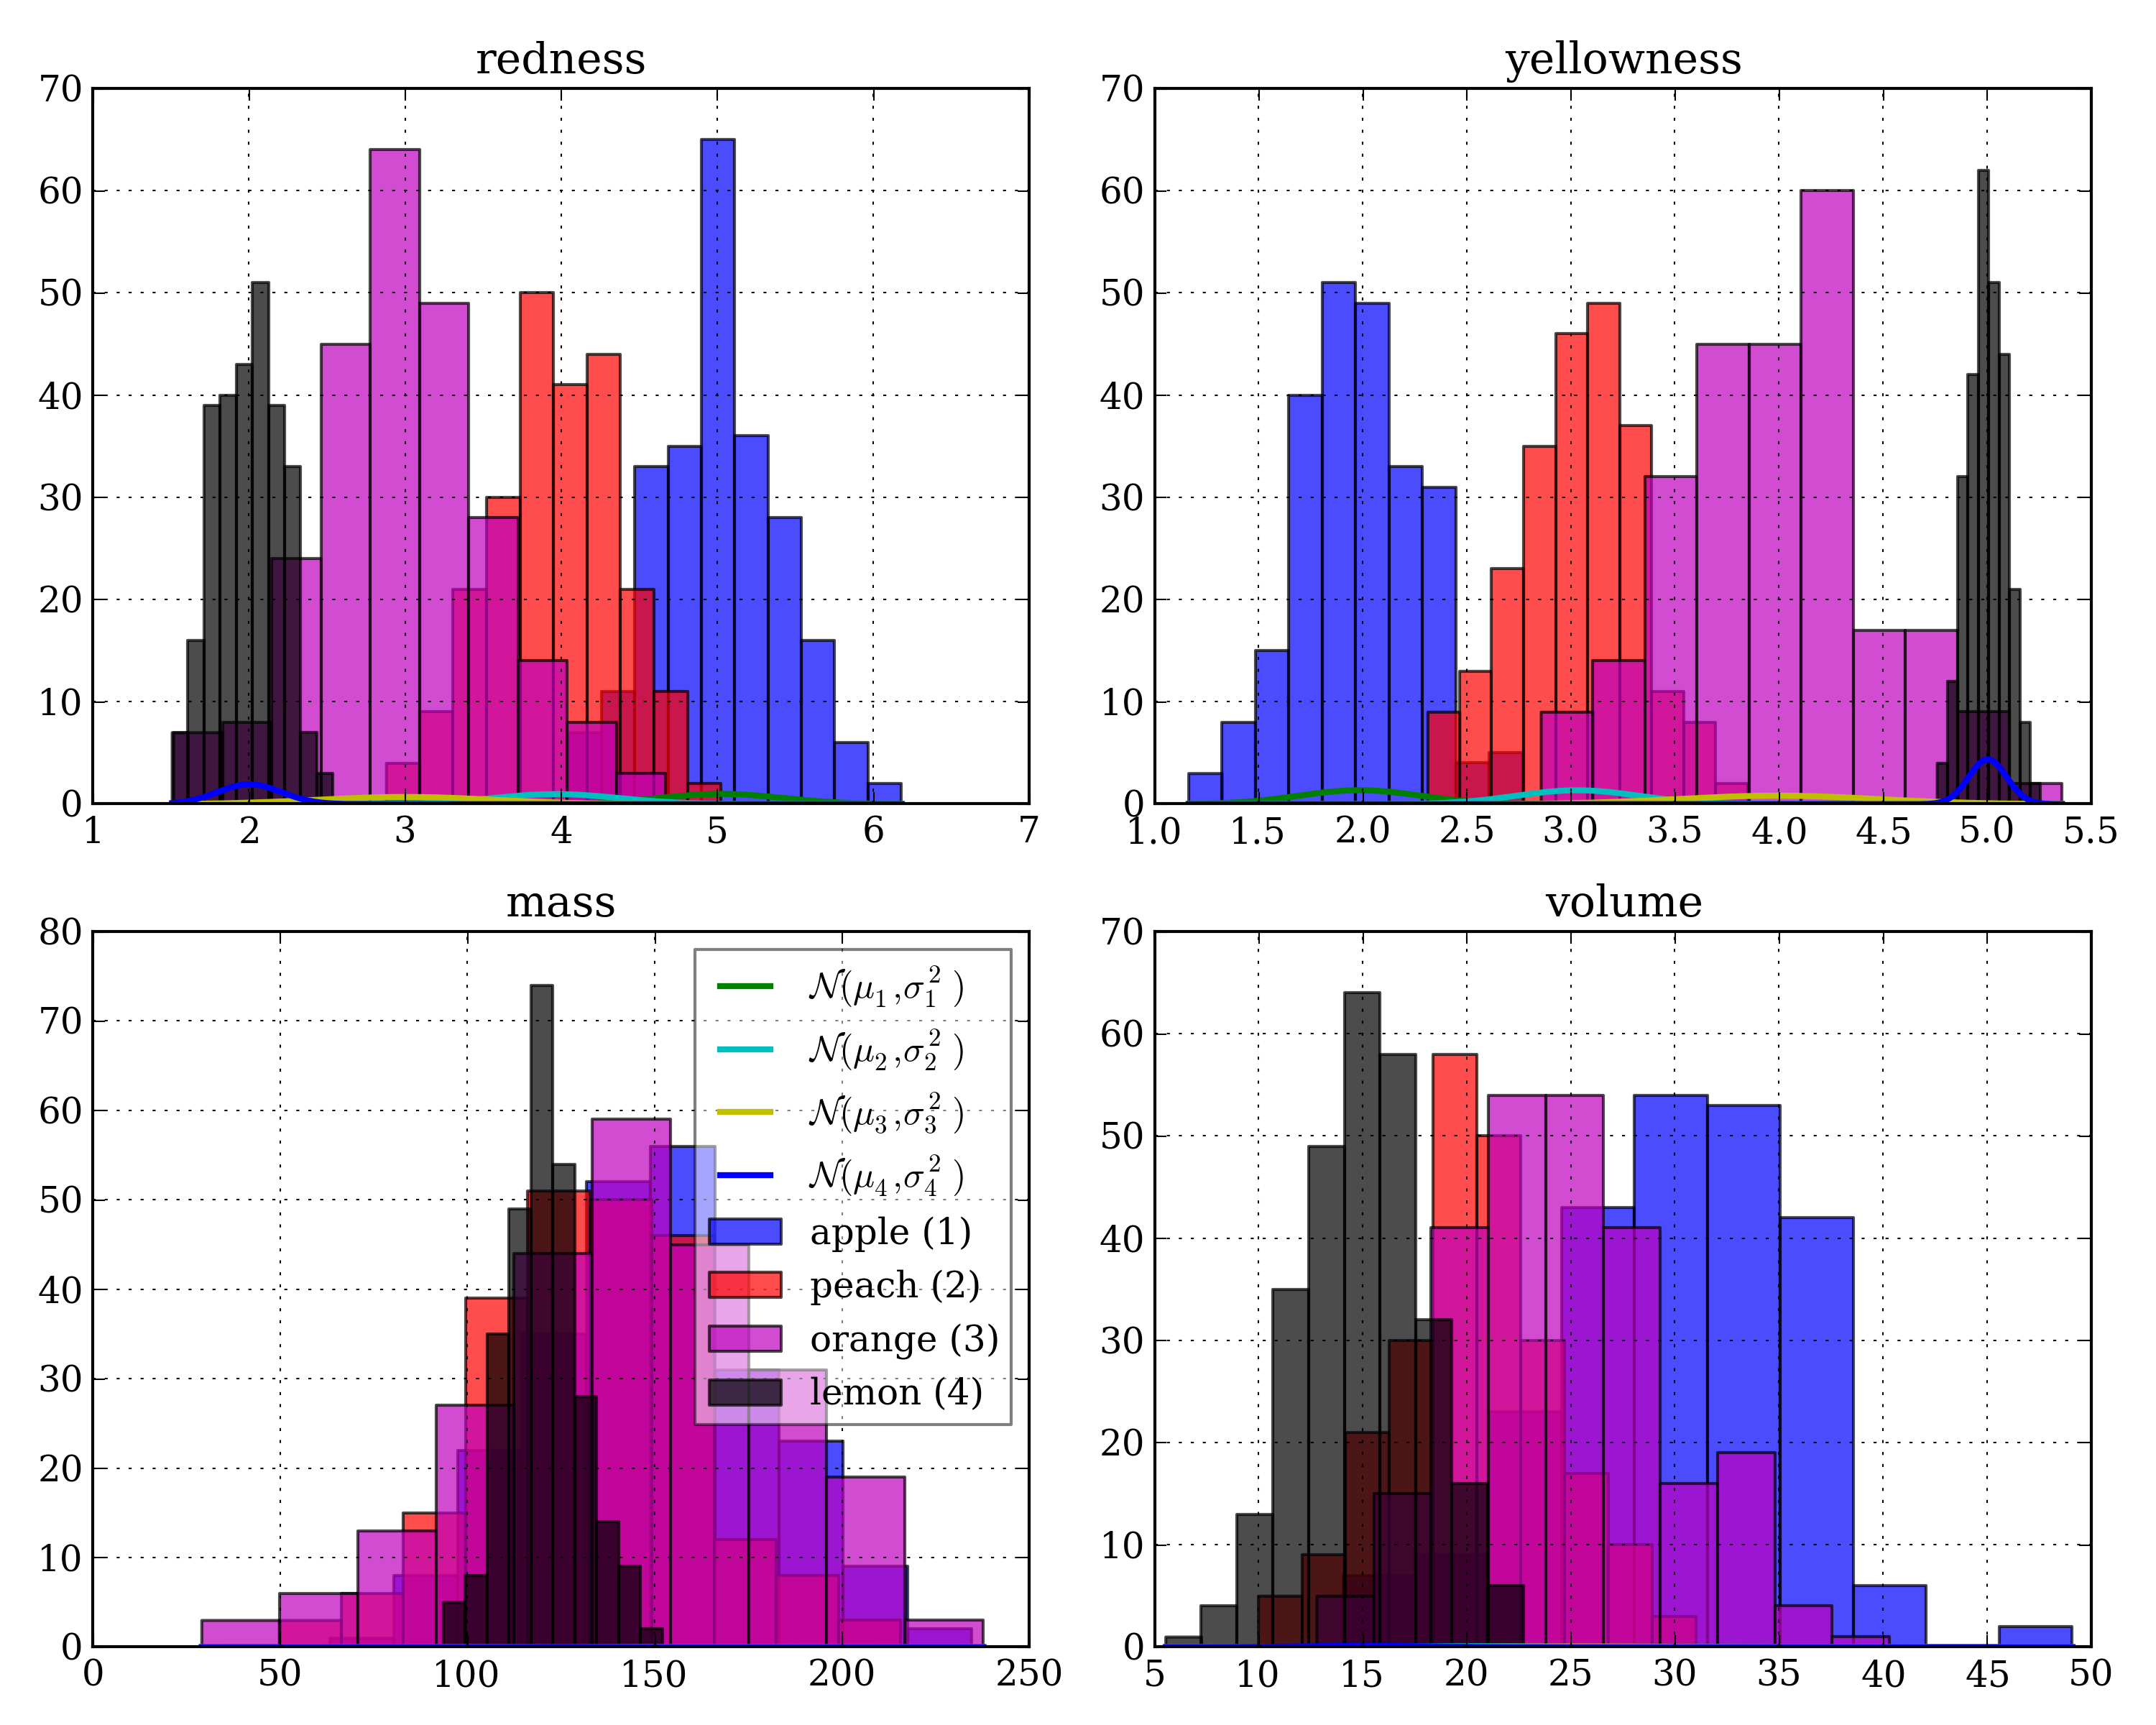
\includegraphics[width=0.4\textwidth]{images/not_normed_original.png}
  \caption{\scriptsize The original data set provided for the project without normalization.  Note that the number of observations for each different fruit are about the same.  The results of Naive Bayes classification are shown below, where the absolute value of the difference between the actual fruit type $v, v_j \in [1,2,3,4]$ is taken from the predicted fruit type.}
\end{figure}

\begin{figure}[H]
  \centering
		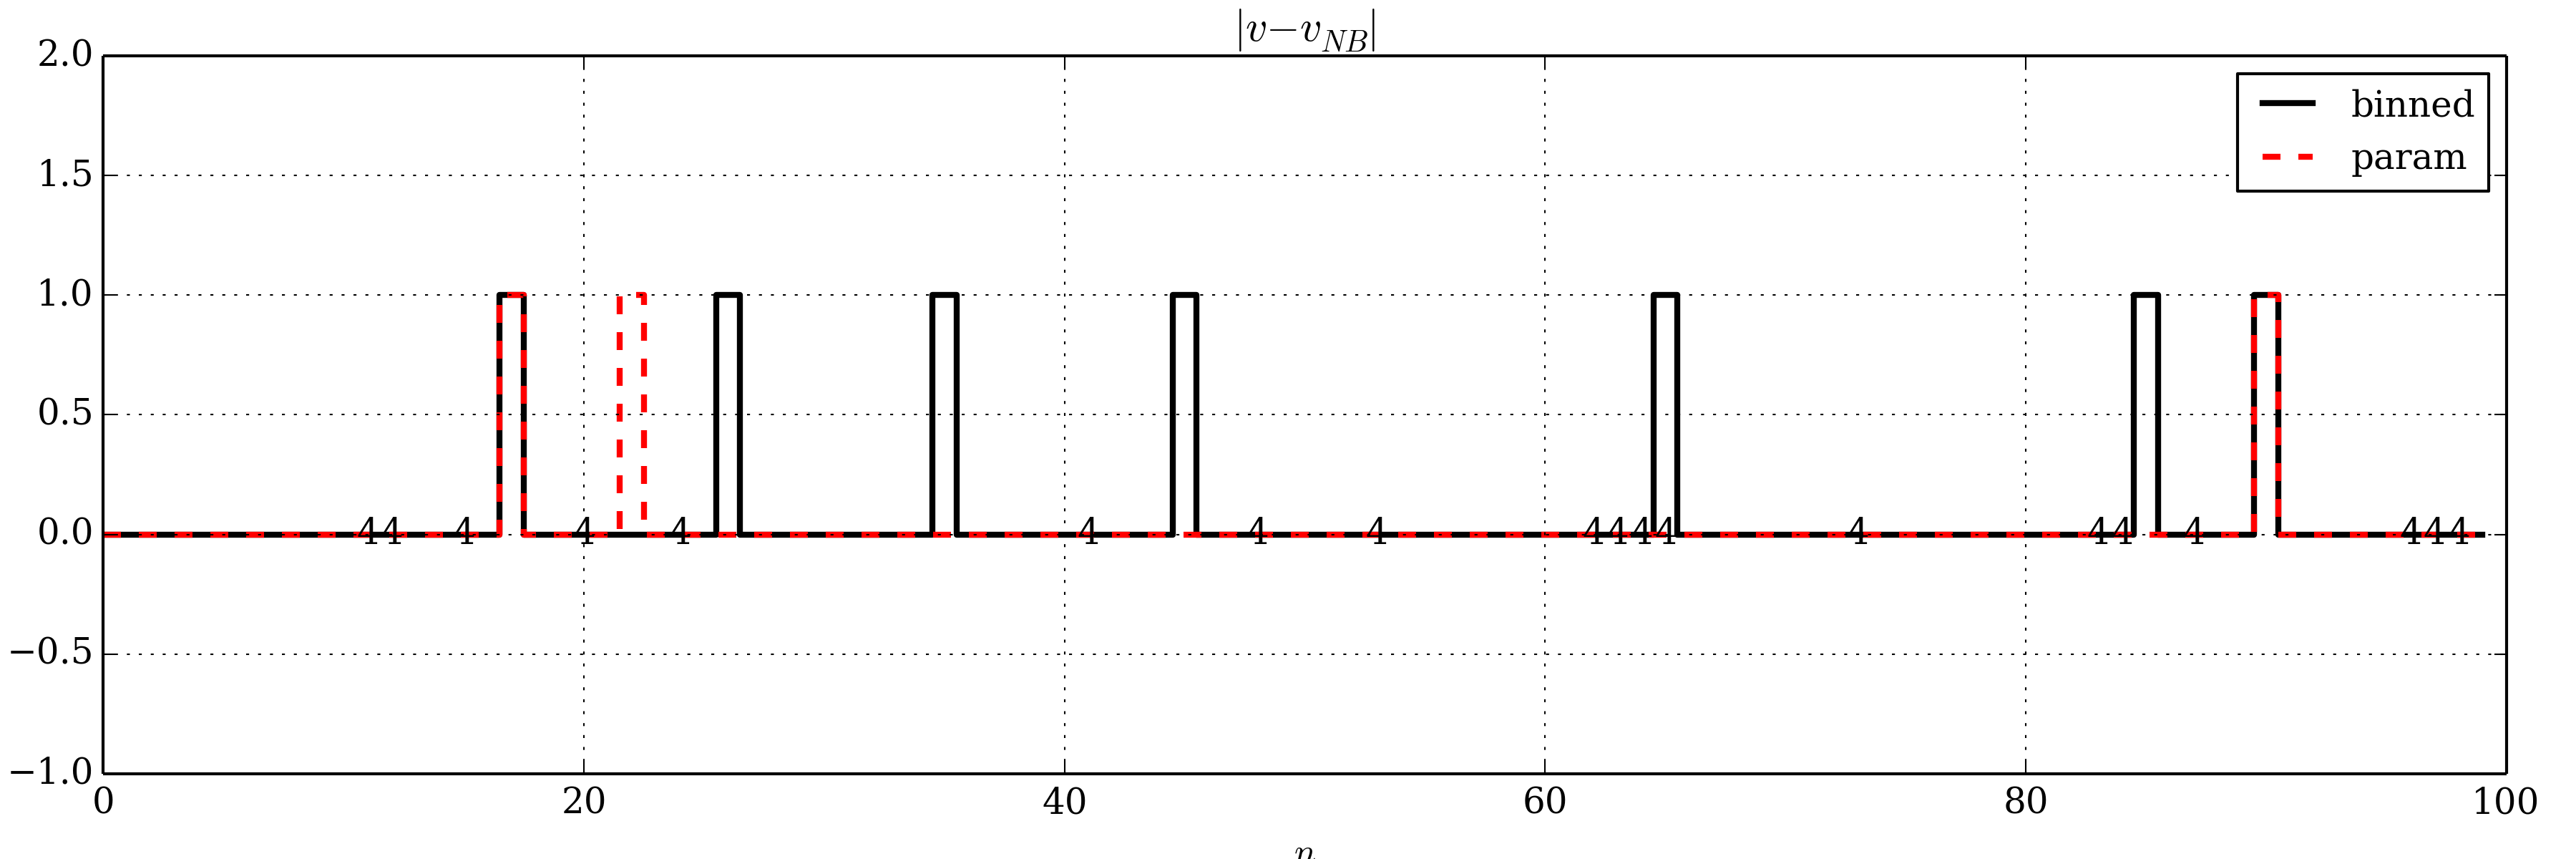
\includegraphics[width=0.4\textwidth]{images/not_normed_original_results.png}
\end{figure}

\begin{figure}[H]
  \centering
		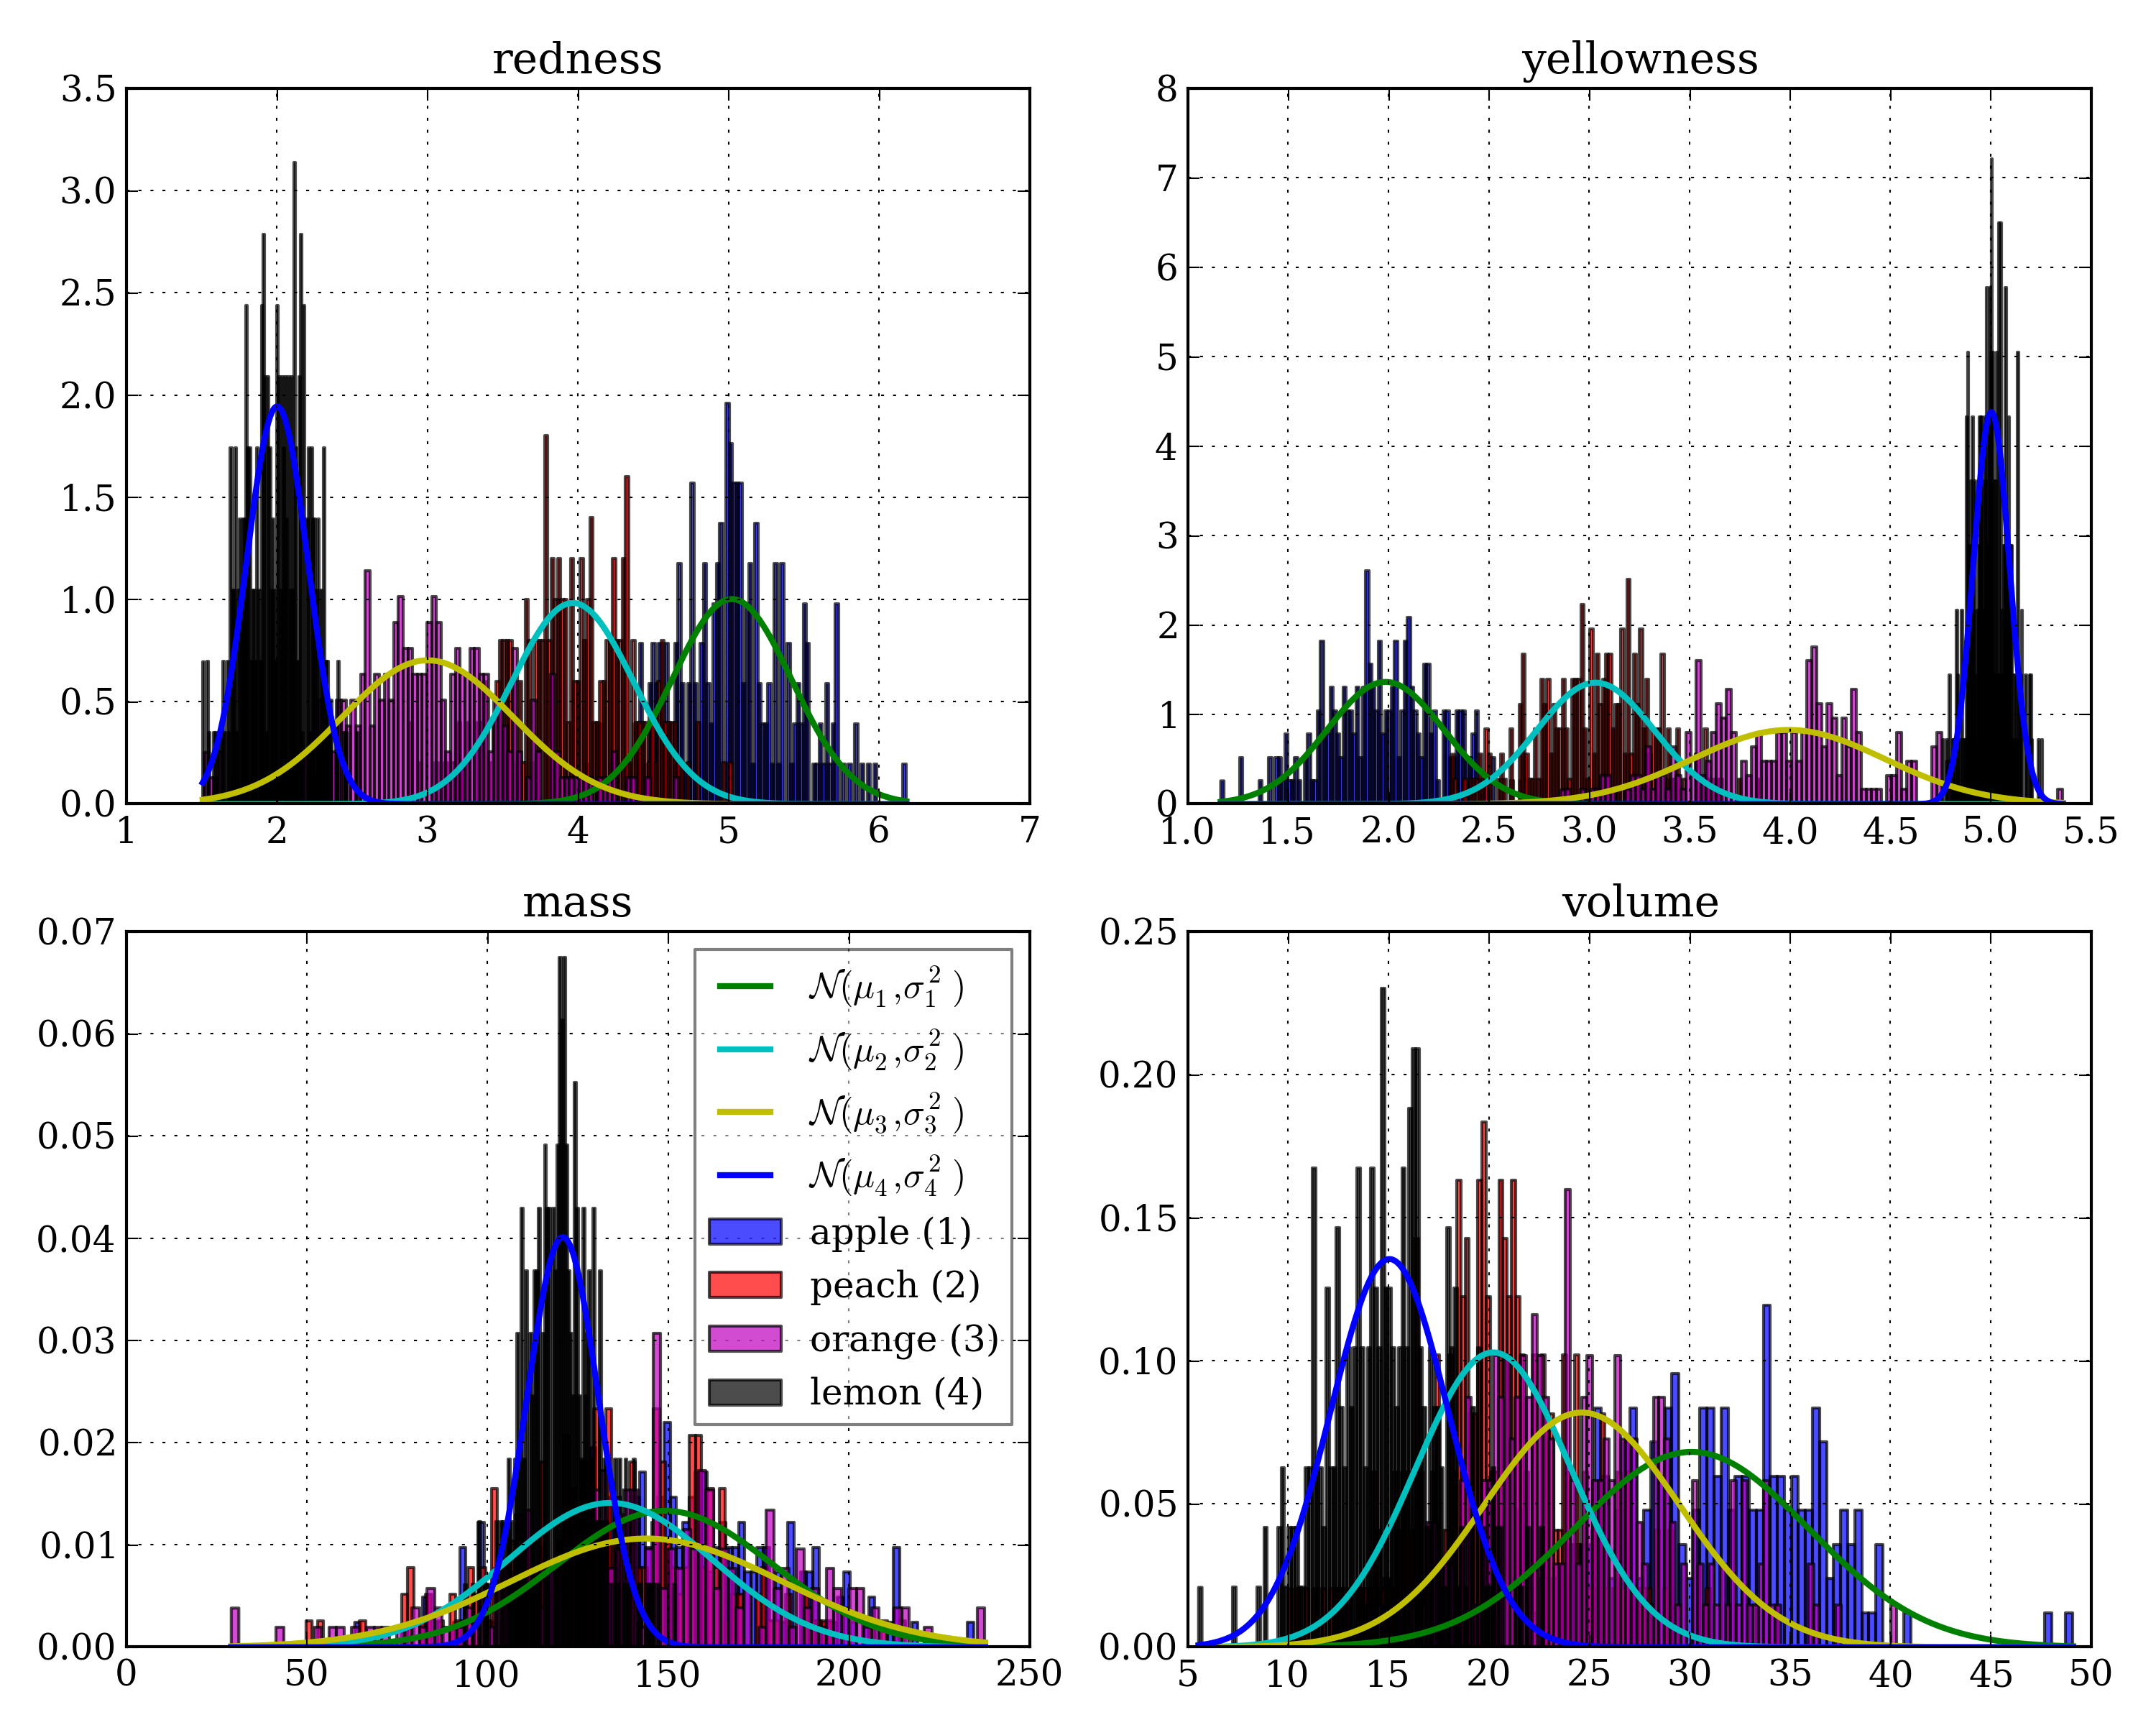
\includegraphics[width=0.4\textwidth]{images/normed_original.png}
  \caption{\scriptsize The original data set with normalization performed.  Notice below the results are about the same.}
\end{figure}

\begin{figure}[H]
  \centering
		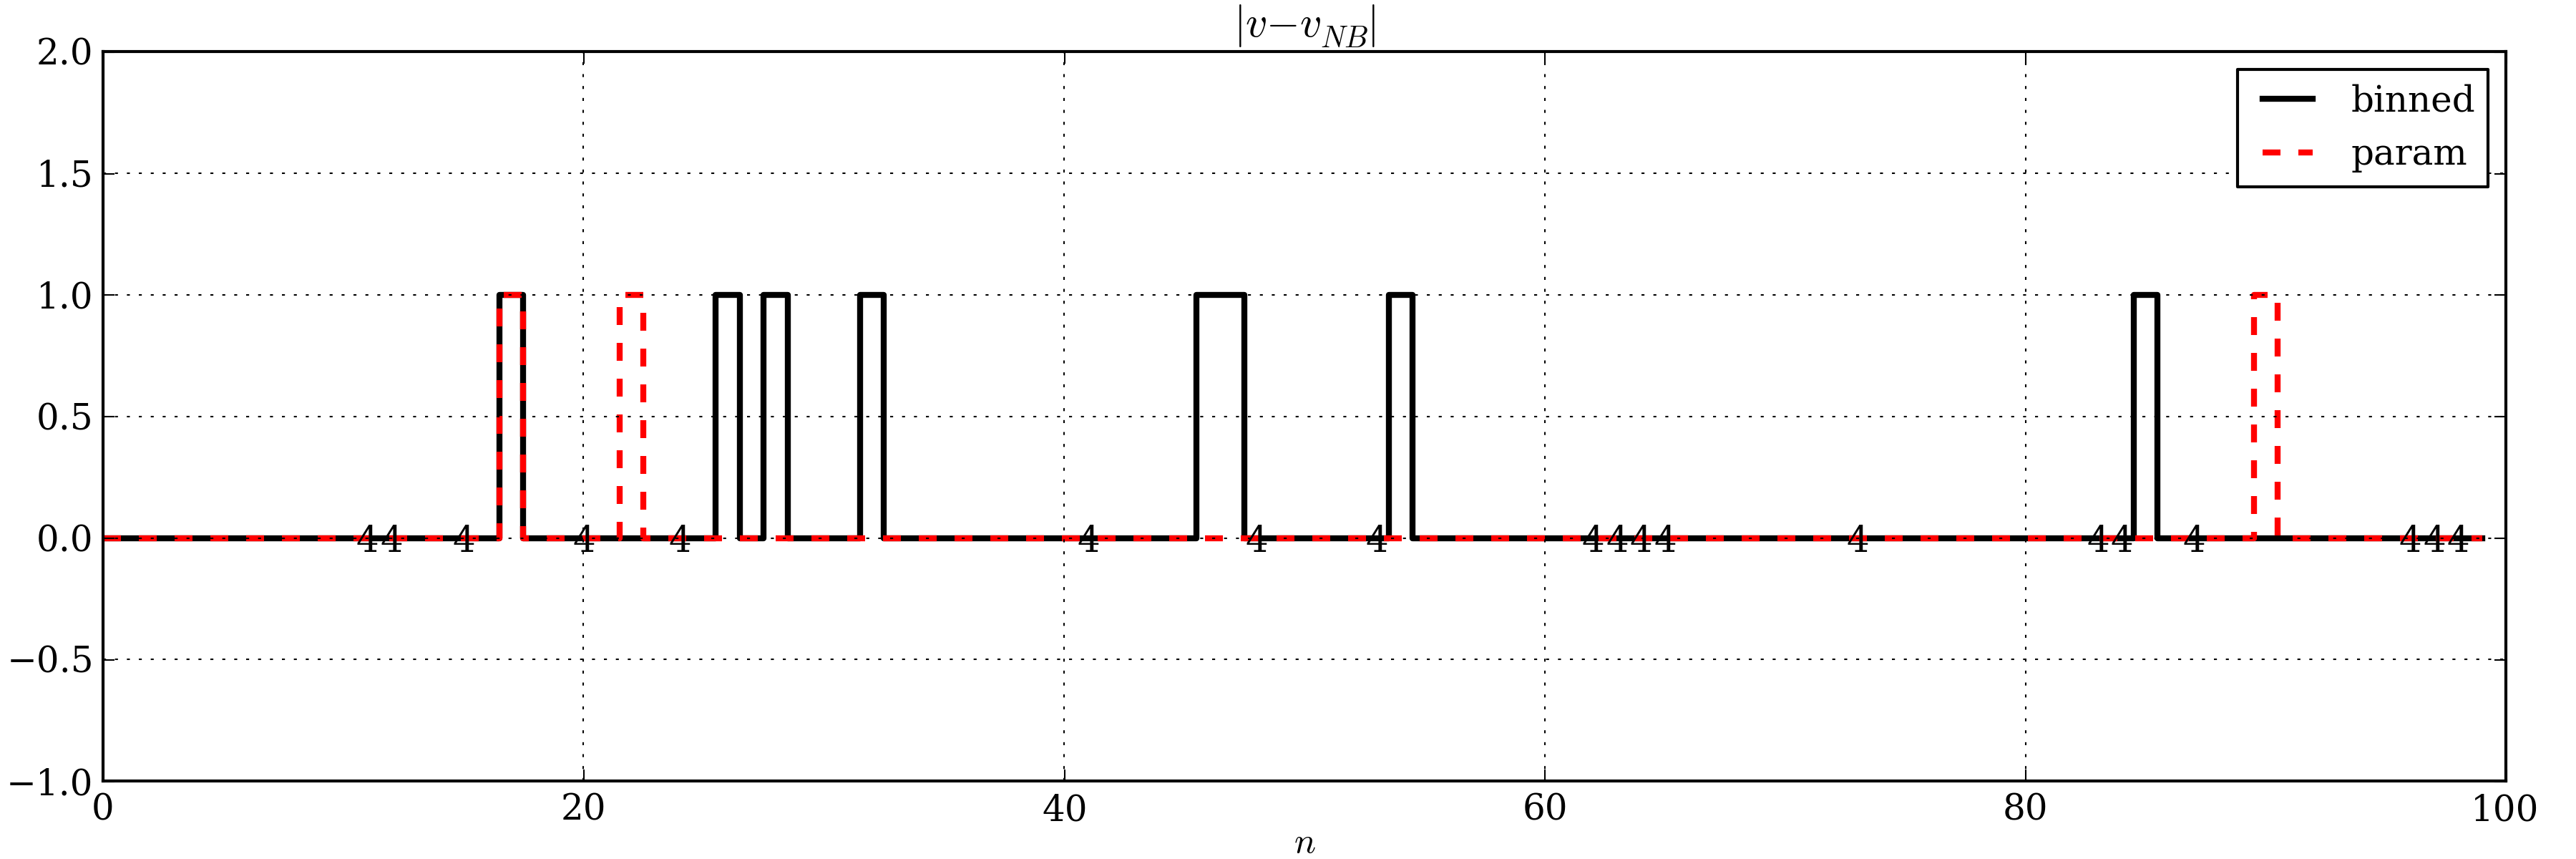
\includegraphics[width=0.4\textwidth]{images/normed_original_results.png}
\end{figure}

\end{multicols}
\begin{multicols}{2}

\begin{figure}[H]
  \centering
		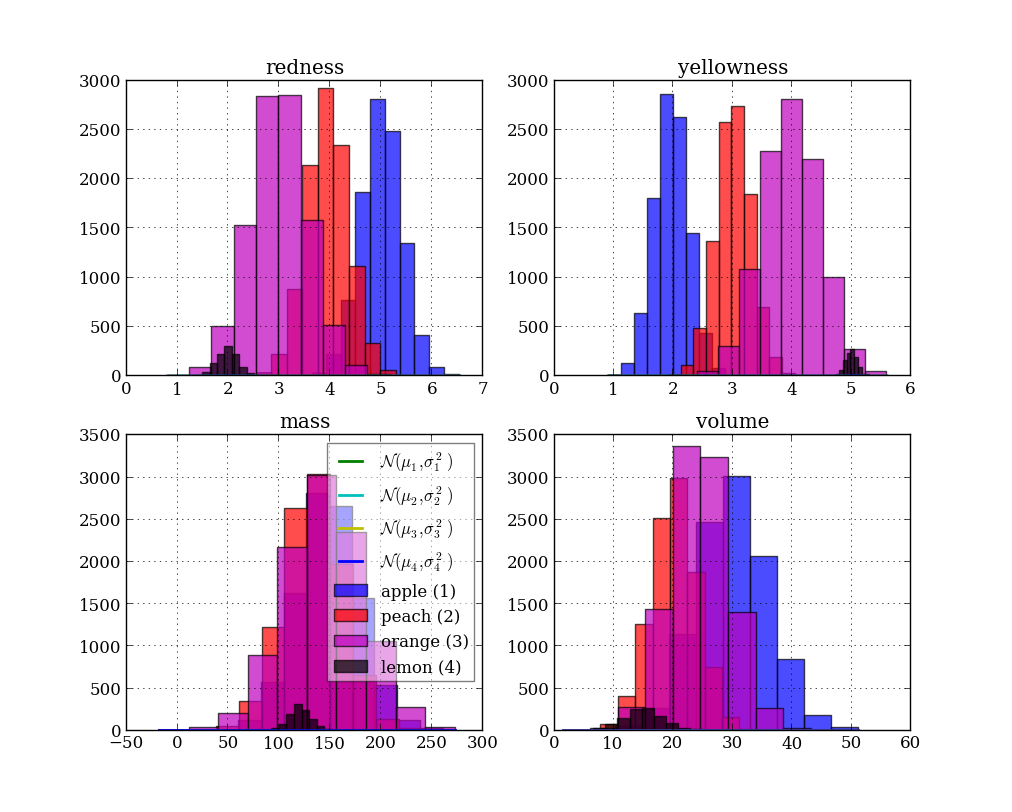
\includegraphics[width=0.4\textwidth]{images/not_normed_new.png}
  \caption{\scriptsize A new data set with the same $\mu$ and $\sigma$ values as the original data, but with 10,000 observations for each fruit except lemons which have 1,000.  Notice that there are a great many 4's (lemons) in the below results which were improperly classified.}
\end{figure}

\begin{figure}[H]
  \centering
		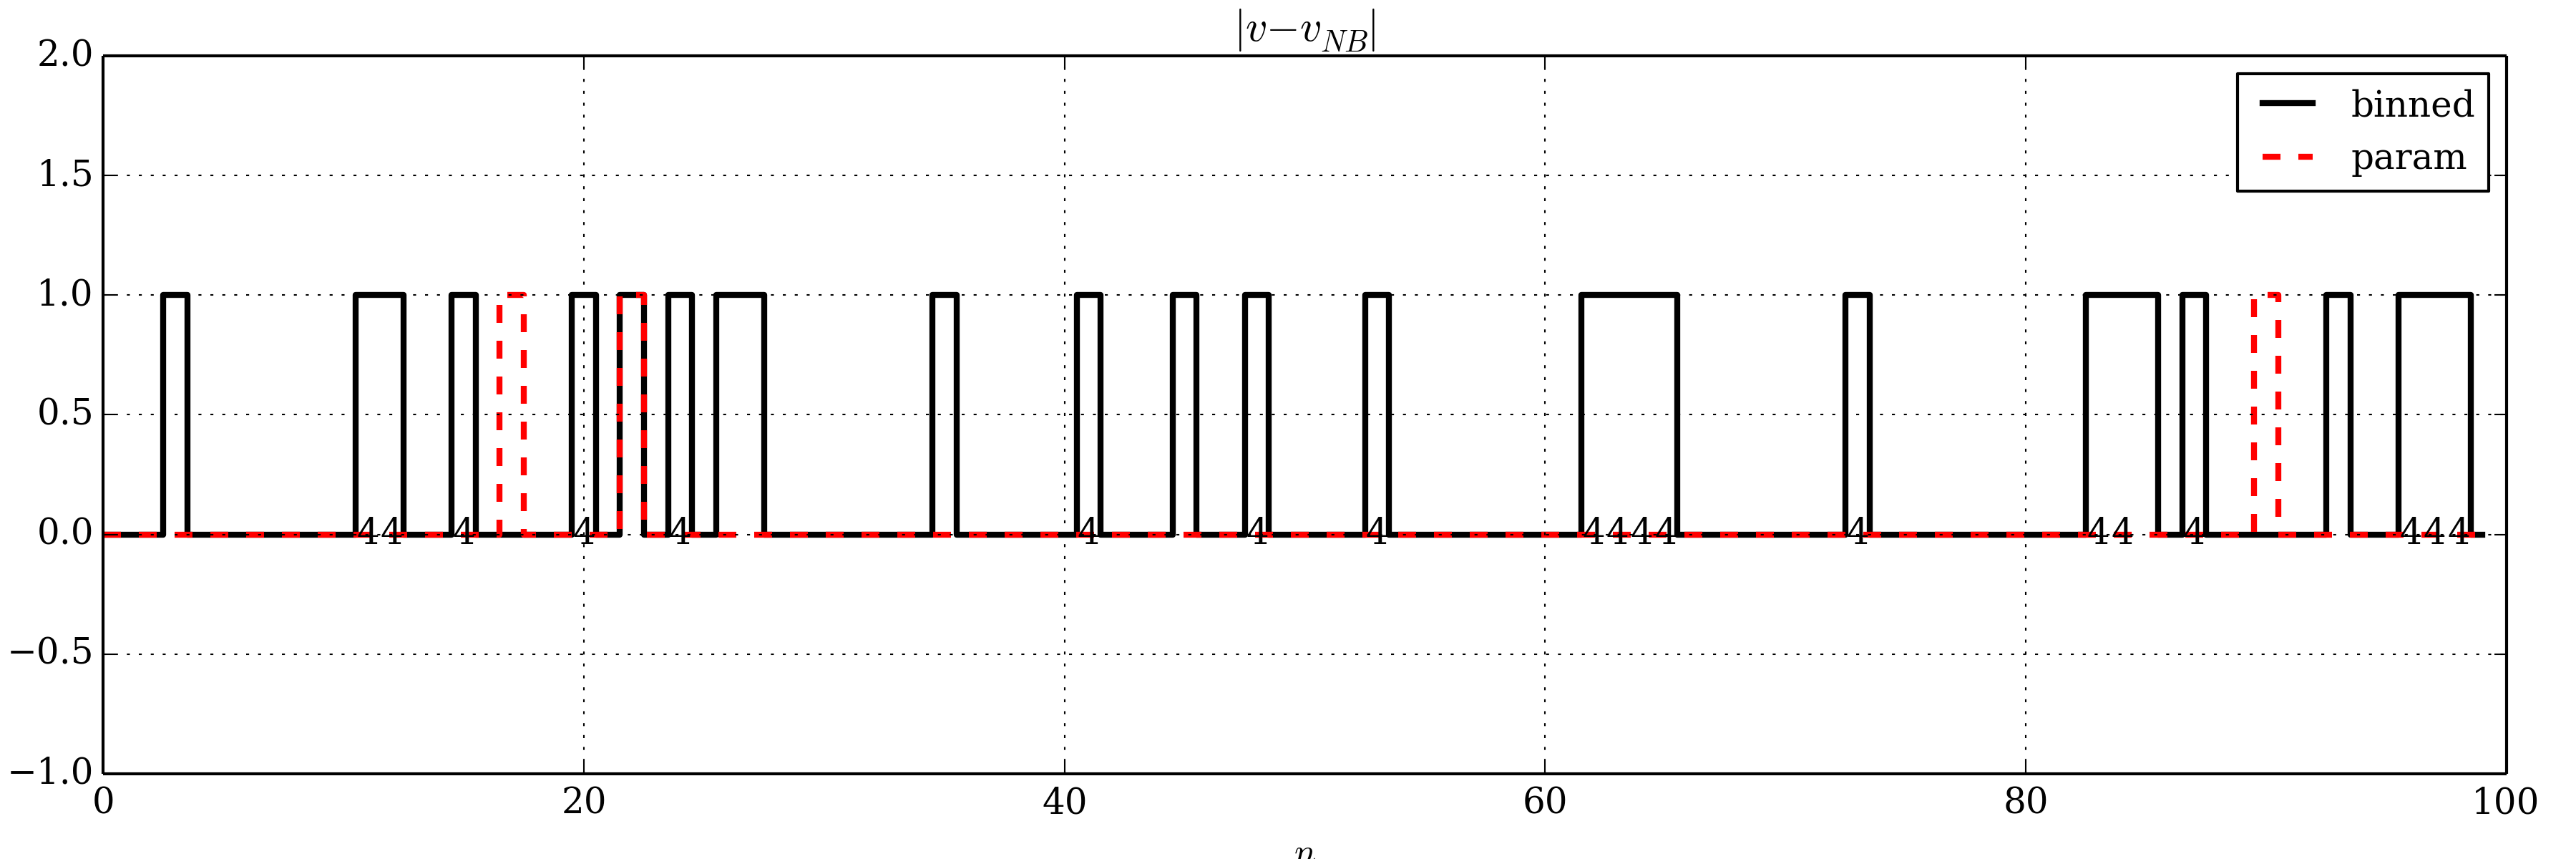
\includegraphics[width=0.4\textwidth]{images/not_normed_new_results.png}
\end{figure}

\begin{figure}[H]
  \centering
		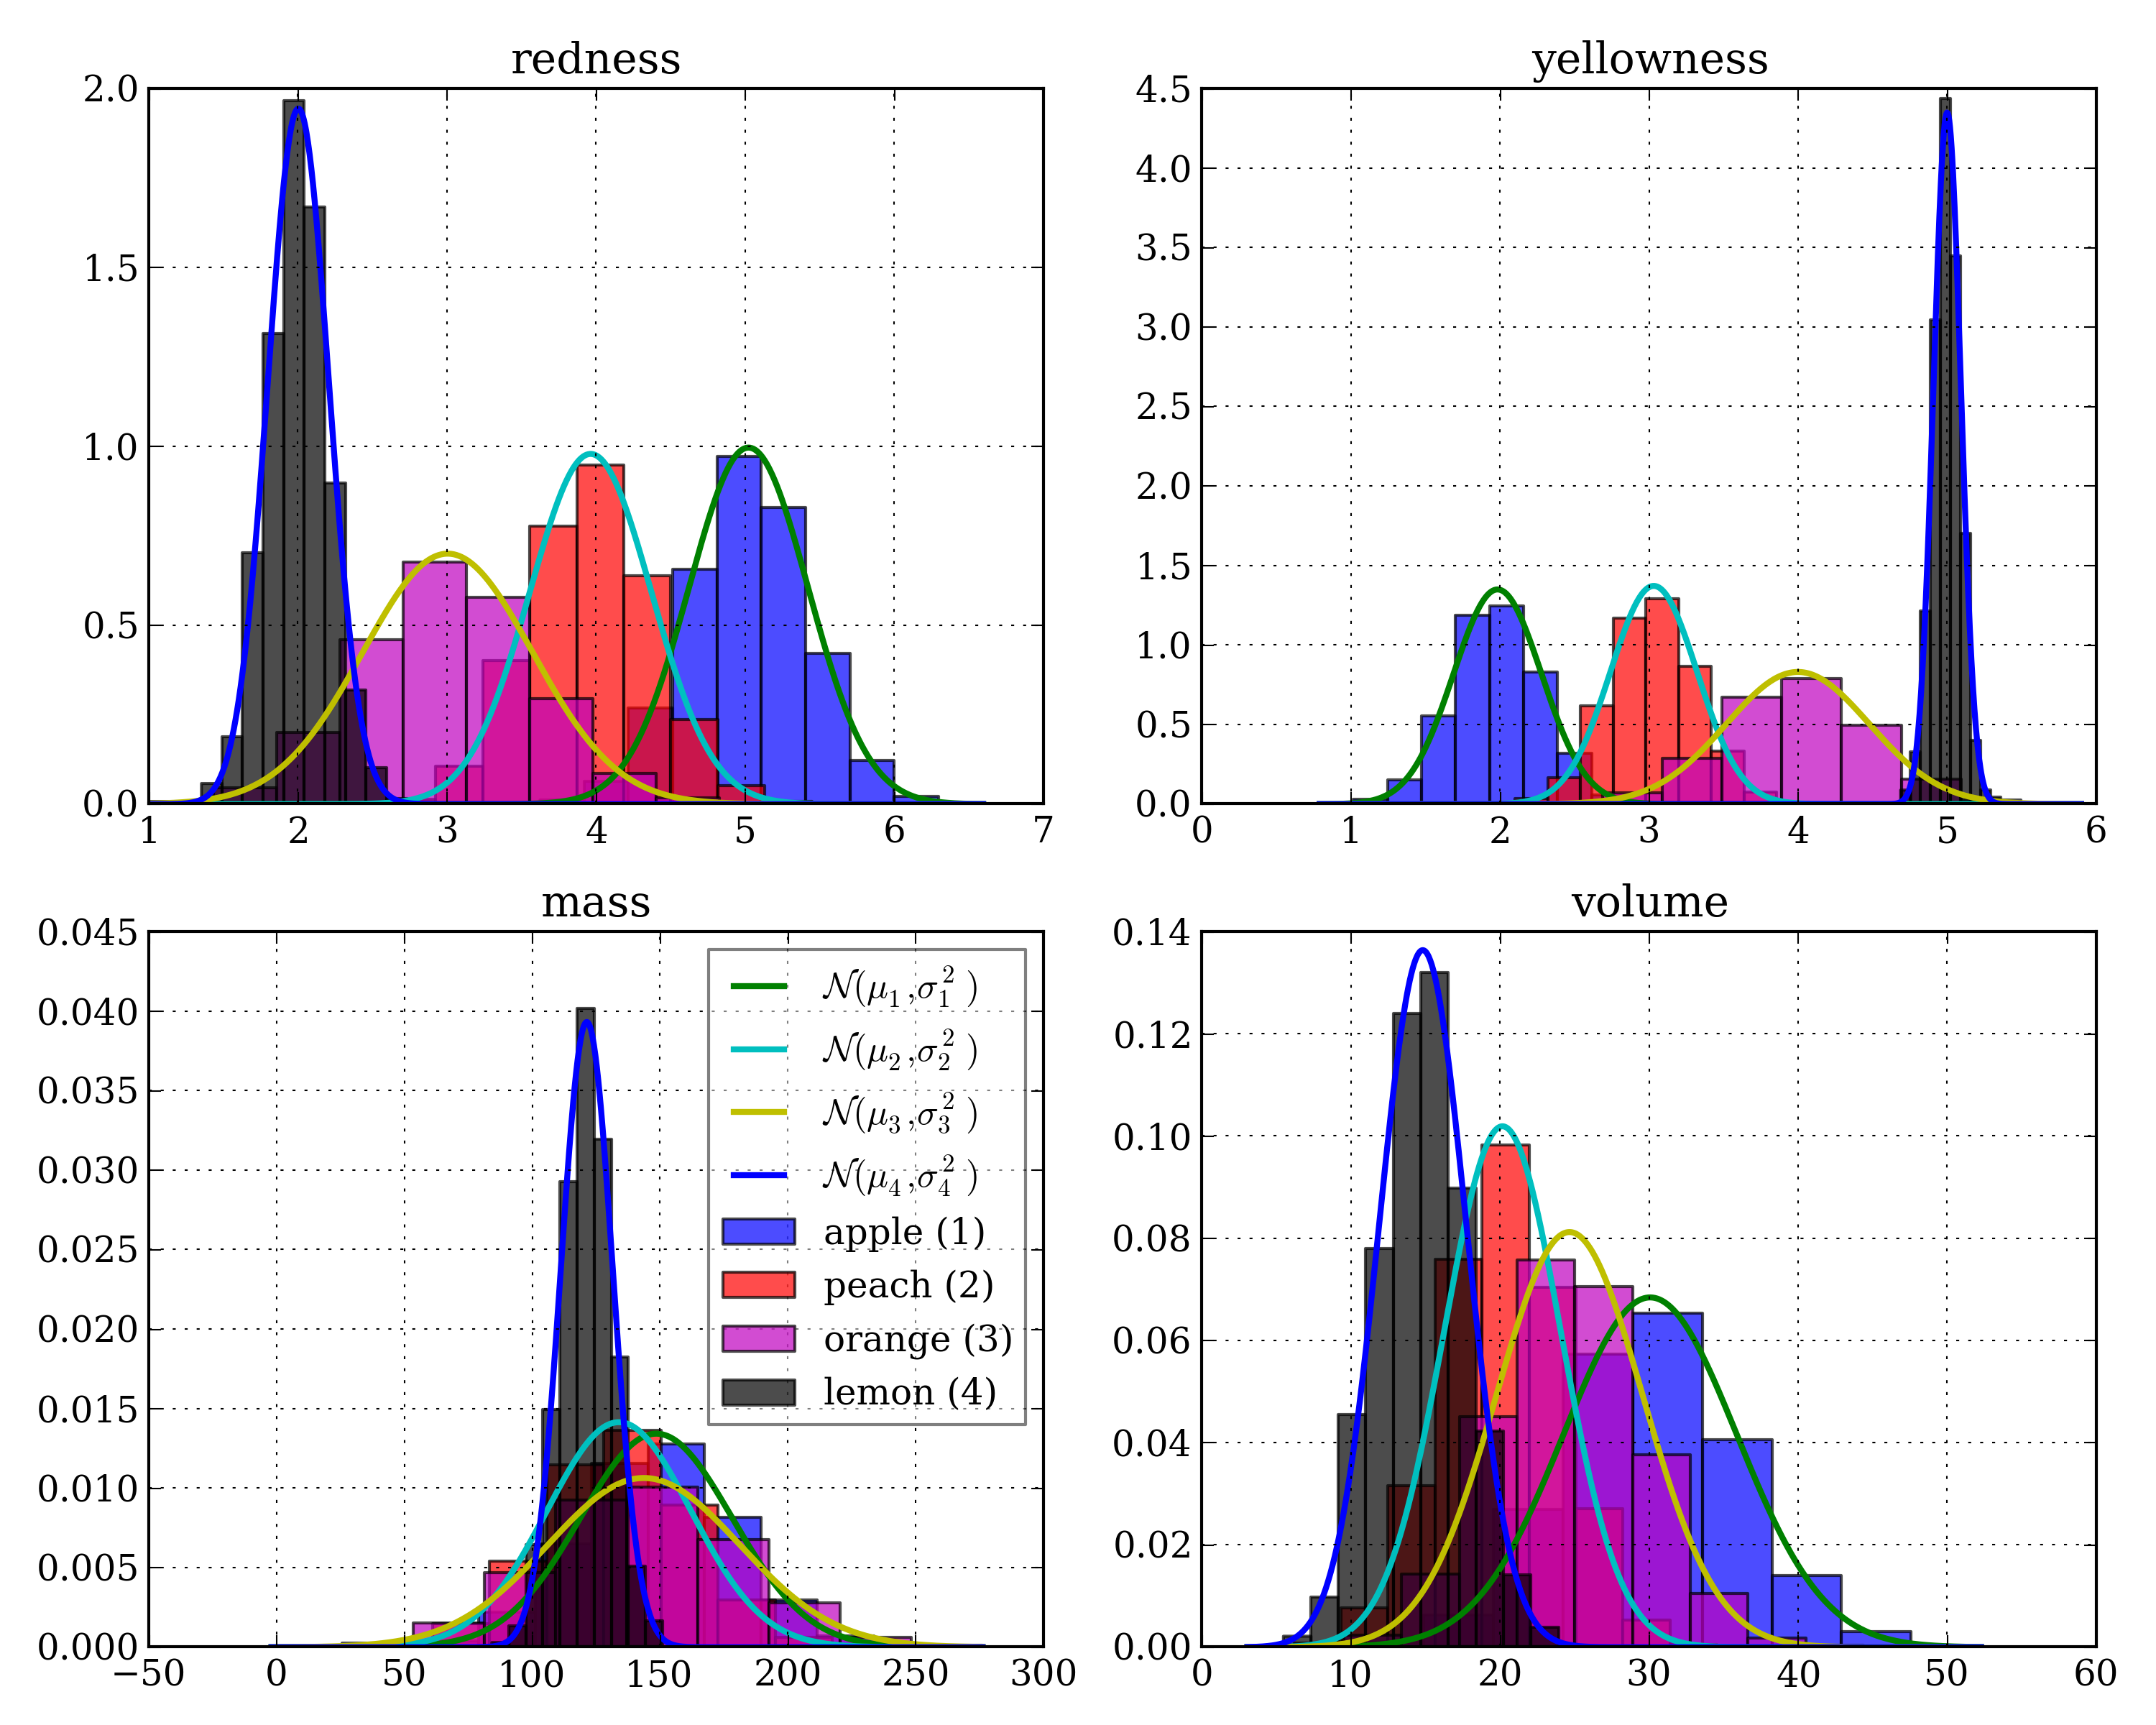
\includegraphics[width=0.4\textwidth]{images/normed_new.png}
  \caption{\scriptsize The same data set as in Figure 3 but with the data normalized.  Note that the results are about the same as Figure 3.  However, if we adjust $P(v_j)$ in Equation (1) to be equal for all $j$, similar results to the parametric approach may be obtained.  See Figure (5).}
\end{figure}

\begin{figure}[H]
  \centering
		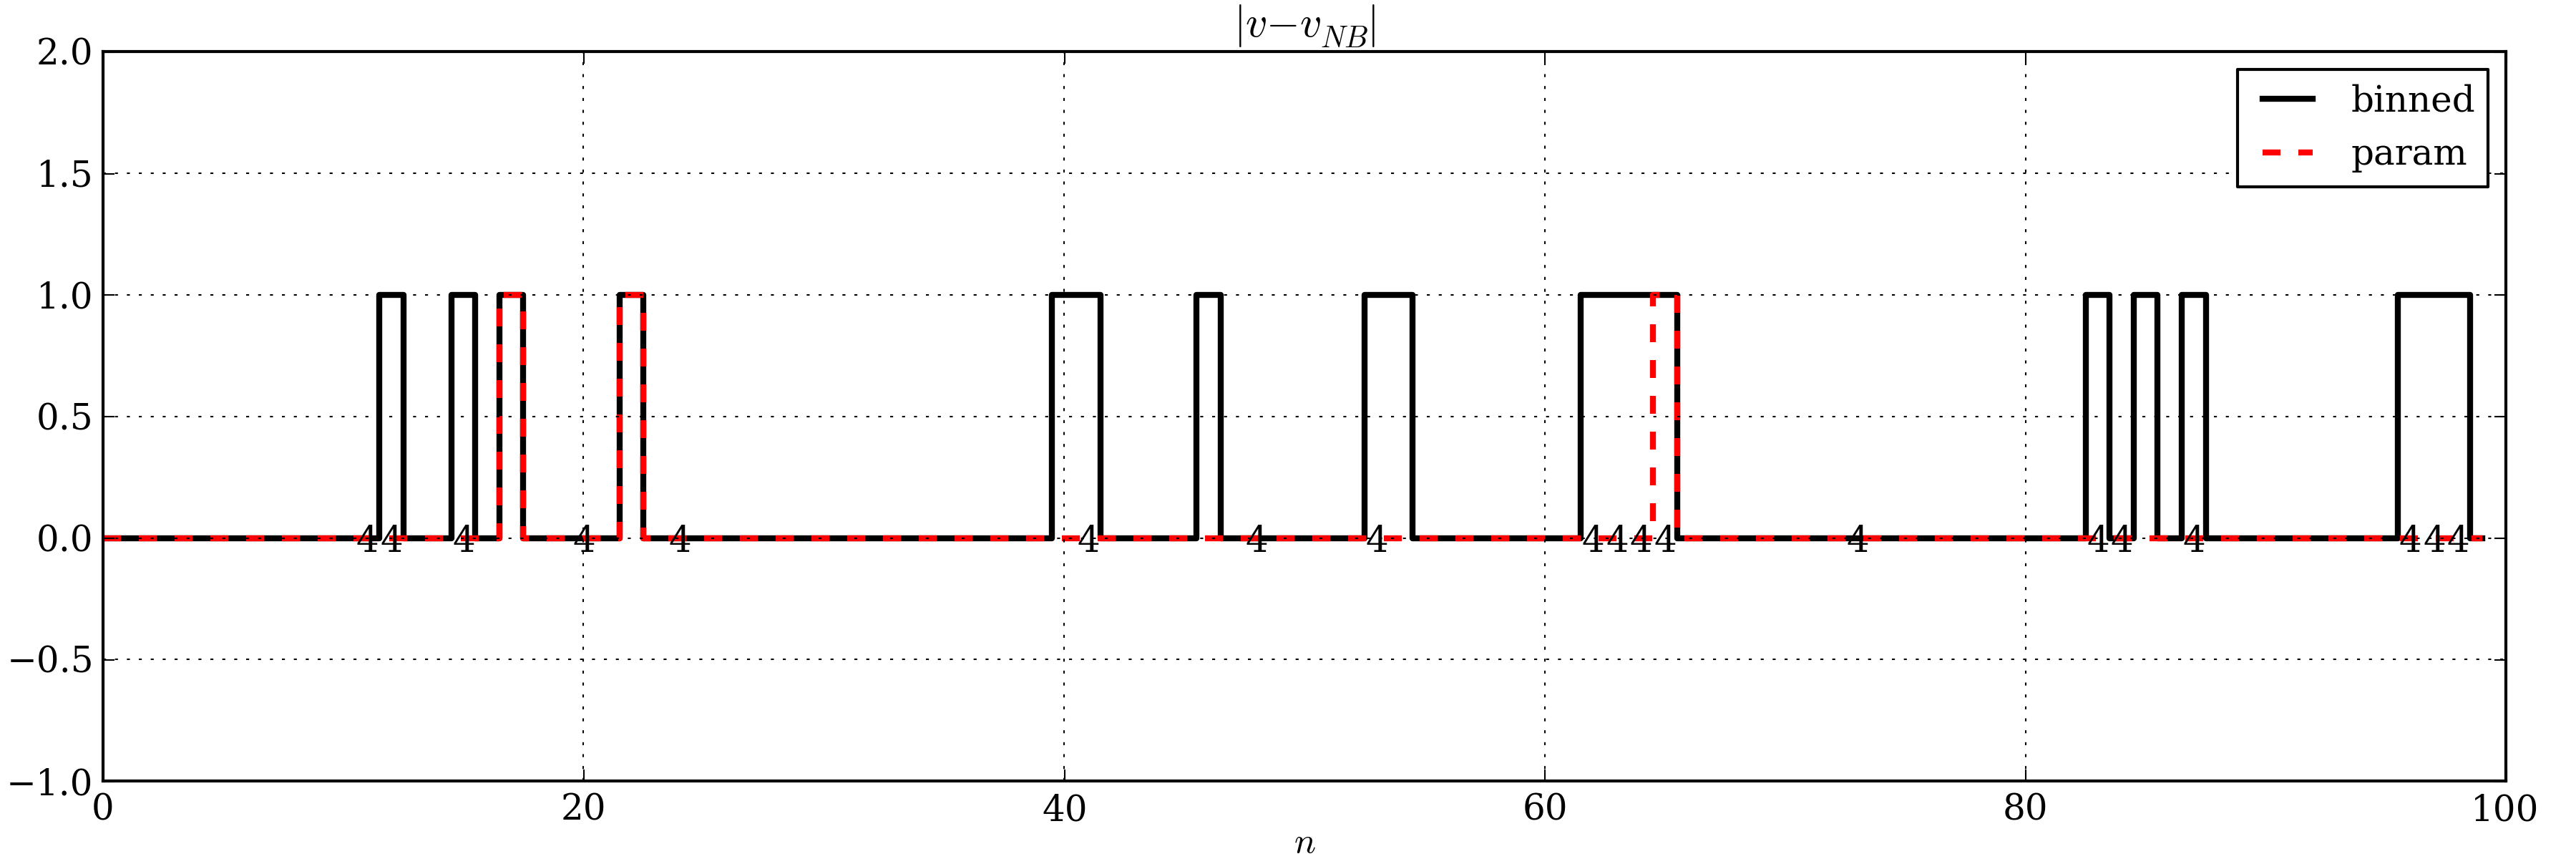
\includegraphics[width=0.4\textwidth]{images/normed_new_results.png}
\end{figure}

\end{multicols}

\newpage

\begin{figure}[H]
  \centering
		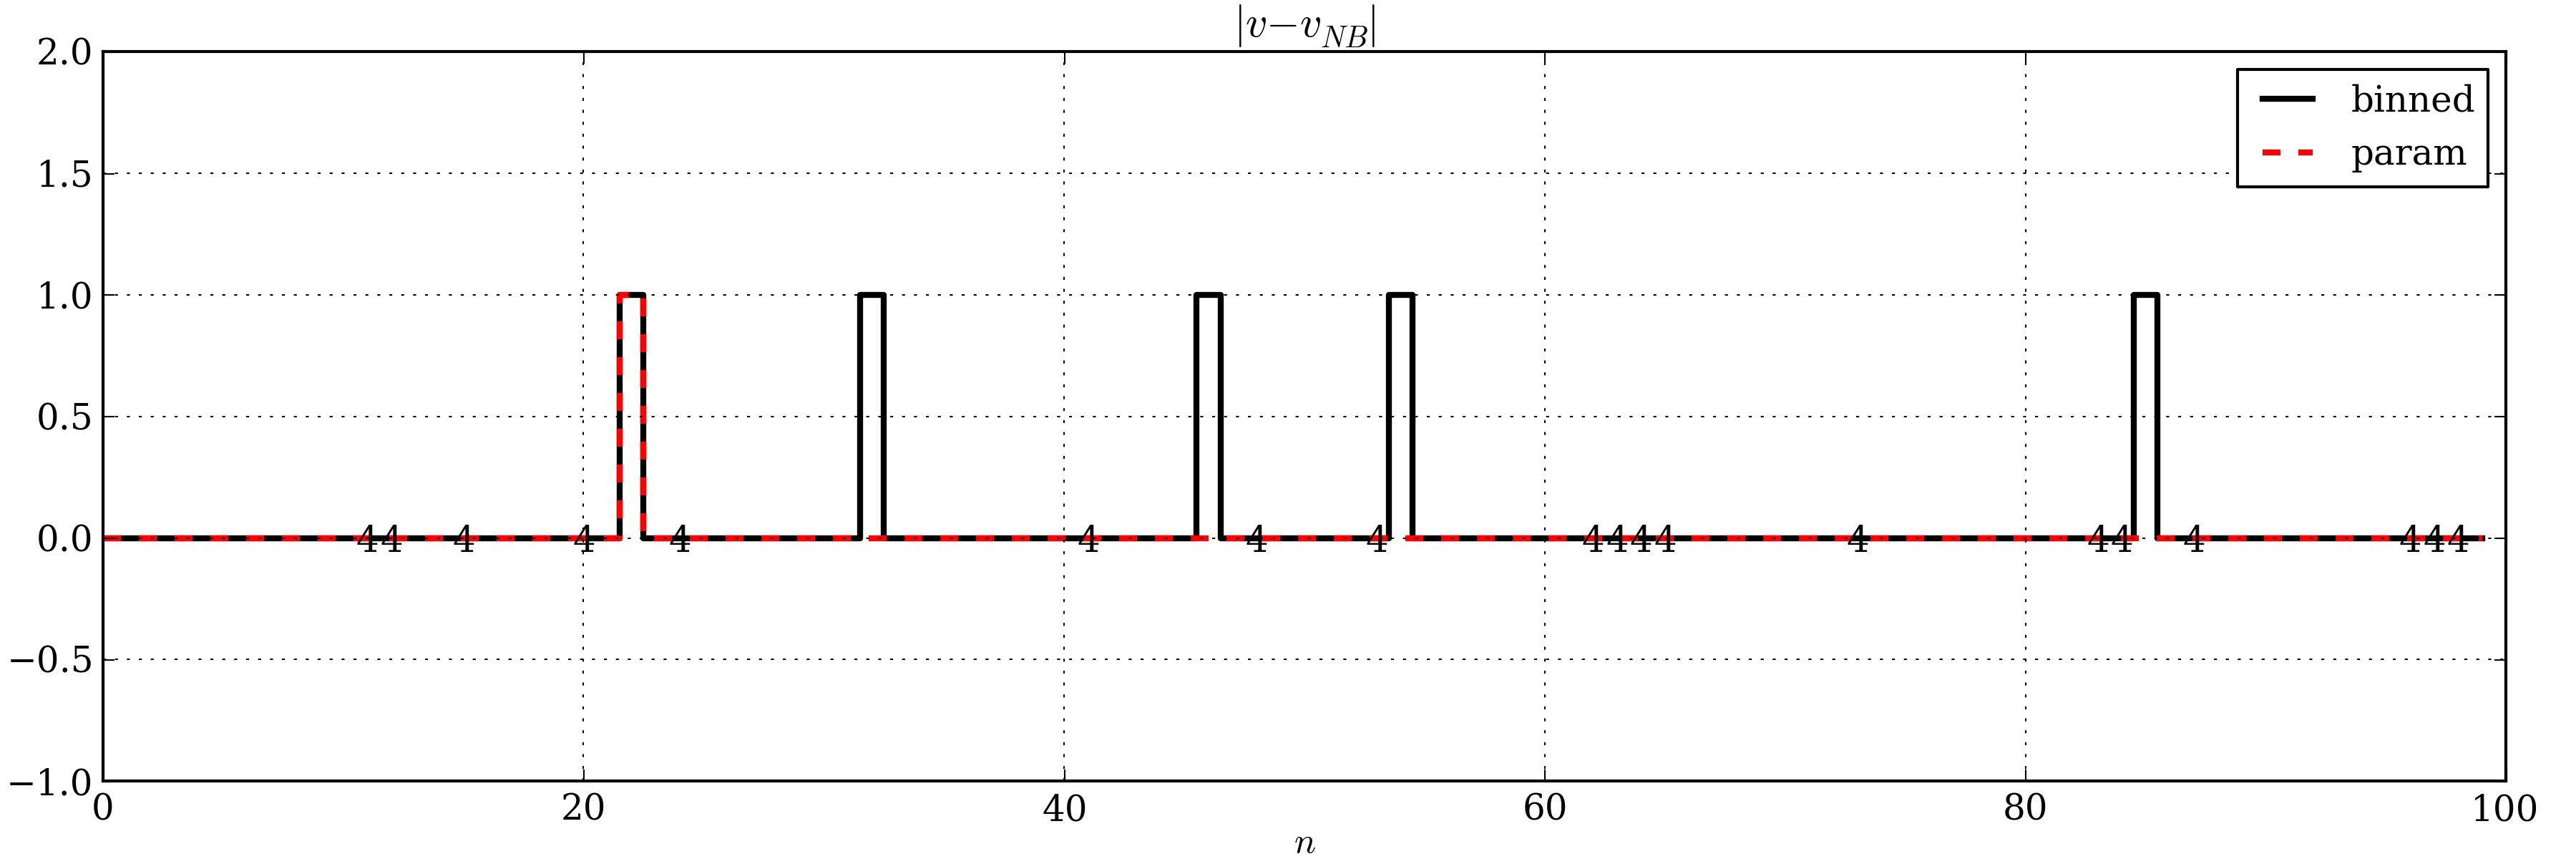
\includegraphics[width=1.0\textwidth]{images/normed_new_results_fixed_prob.png}
  \caption{\scriptsize Results for the N.B.\ classification with adjusted $P(v_j)$ in Equation (1) to be equal for all $j$.  Note the vast improvement from Figure (4).}
\end{figure}

An $m$-estimation scheme has also been utilized for the binned data probabilities.  This converts the probabilities into

$$P(a_i | v_j) = \frac{n_{v_i} + mp}{n + m},$$

where $n_{v_i}$ is the number values with attribute $a_i$, $n$ is the total number of values observed with attribute $a_i$, $m$ is the size of the training set, and $p=1/m$.  This scheme removes difficulties which arise when $n_c$ or $n$ is zero.  The results using non-normalized and normalized data, along with their parametric counterparts are shown below.

\begin{table}[H]
\parbox{.45\linewidth}
{
  \centering
  \begin{tabular}{ c | c c c }
    bin size & \specialcell{non-\\normal'd} & normal'd & param. \\
    \hline
    10  & 93 & 92 & 97 \\
    20  & 91 & 93 & 97 \\
    50  & 88 & 89 & 97 \\
    100 & 88 & 92 & 97 \\
  \end{tabular}
  \caption{Results for the original data set.}
  \label{tbl:tablelabel}
}
\hfill
\parbox{.45\linewidth}
{
  \centering
  \begin{tabular}{ c | c c c }
    bin size & \specialcell{non-\\normal'd} & normal'd & param. \\
    \hline
    10  & 75 & 80 & 98 \\
    20  & 73 & 82 & 97 \\
    50  & 74 & 81 & 99 \\
    100 & 75 & 81 & 98 \\
  \end{tabular}
  \caption{Results for the new data set.}
  \label{tbl:tablelabel}
}
\end{table}

\begin{table}[H] 
\centering
\begin{tabular}{ c | c c c }
  bin size & \specialcell{non-\\normal'd} & normal'd & param. \\
  \hline
  10  & 76 & 89 & 98 \\
  20  & 75 & 93 & 99 \\
  50  & 73 & 91 & 97 \\
  100 & 72 & 91 & 99 \\
\end{tabular}
\caption{Results for the new data set with $P(v_j) = P(v_i)$.}
\label{tbl:tablelabel}
\end{table}

\subsection*{Discussion}

Table (2) shows that even with the normalization, the accuracy is still less than the parametrized estimate.  This is due to the fact that the value $P(v_j)$ in Equation (1) down-weights the values with low numbers of observations.  See Figure (5) and Table (3) for the results with $P(v_j) = P(v_i)\ \forall\ i,j \in [1,m]$.

Please note that if this is worth publishing, the results with probabilities not adjusted would not be provided.  This has been included as part of the development process.
 

\end{document}




